% DO NOT COMPILE THIS FILE DIRECTLY!
% This is included by the other .tex files.

\begin{frame}
\titlepage
\end{frame}

\begin{frame}
  \frametitle{The aim of this presentation}
  \begin{itemize}
     \item Why is {\bf contextualisation} important?
     \item What options do we have in MISP?
     \item How can we {\bf leverage} this in the end?
  \end{itemize}
\end{frame}


\begin{frame}
\frametitle{The growing need to contextualise data}
\begin{itemize}
       \item Contextualisation became more and more important as we as a community matured
        \begin{itemize}
                \item {\bf Growth and diversification} of our communities
                \item Distinguish between information of interest and raw data
                \item {\bf False-positive} management
                \item TTPs and aggregate information may be prevalent compared to raw data (risk assessment)
                \item {\bf Increased data volumes} leads to a need to be able to prioritise
	\end{itemize}
	\item These help with filtering your TI based on your {\bf requirements}...
	\item ...as highlighted by Pasquale Stirparo \textit{Your Requirements Are Not My Requirements}
\end{itemize}
\end{frame}

\begin{frame}
\frametitle{Objectives}
\begin{itemize}
       \item Some main objectives we want to achieve when producing data
        \begin{itemize}
                \item Ensure that the information is {\bf consumable} by everybody
                \item That it is {\bf useful} to the entire target audience
                \item The data is {\bf contextualised} for it to be understood by everyone
	\end{itemize}
        \item What we ideally want from our data
        \begin{itemize}
                \item We want to be able to {\bf filter} data for different use-cases
                \item We want to be able to get as much knowledge out of the data as possible
                \item We want to know where the data is from, how it got there, why we should care
	\end{itemize}
\end{itemize}
\end{frame}

\begin{frame}
\frametitle{Different layers of context}
\begin{itemize}
       \item Context added by analysts / tools
       \item Data that tells a story
       \item Encoding analyst knowledge to automatically leverage the above
\end{itemize}
\end{frame}

\section{Context added by analysts / tools}

\begin{frame}
\frametitle{Expressing why data-points matter}
\begin{itemize}
       \item An IP address by itself is barely ever interesting
       \item We need to tell the recipient / machine why this is relevant
       \item All data in MISP has a bare minimum required context
       \item We differentiate between indicators and supporting data
\end{itemize}
\end{frame}

\begin{frame}
\frametitle{Broadening the scope of what sort of context we are interested in}
\begin{itemize}
       \item {\bf Who} can receive our data? {\bf What} can they do with it?
       \item {\bf Data accuracy, source reliability}
       \item {\bf Why} is this data relevant to us?
       \item {\bf Who} do we think is behind it, {\bf what tools} were used?
       \item What sort of {\bf motivations} are we dealing with? Who are the {\bf targets}?
       \item How can we {\bf block/detect/remediate} the attack?
       \item What sort of {\bf impact} are we dealing with?
\end{itemize}
\end{frame}

\begin{frame}
\frametitle{Tagging and taxonomies}
\begin{itemize}
       \item Simple labels
       \item Standardising on vocabularies
       \item Different organisational/community cultures require different nomenclatures
       \item Triple tag system - taxonomies
       \item JSON libraries that can easily be defined without our intervention
\end{itemize}
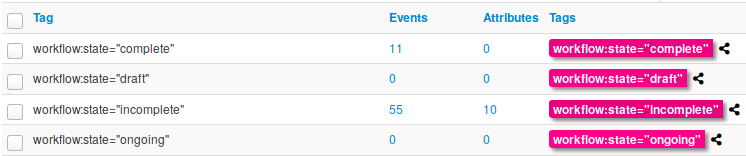
\includegraphics[width=1.0\linewidth]{taxonomy-workflow.png}
\end{frame}

\begin{frame}
\frametitle{Galaxies}
    \begin{itemize}
      \item Taxonomy tags often {\bf non self-explanatory}
      \begin{itemize}
       \item Example: universal understanding of tlp:green vs APT 28
      \end{itemize}
       \item For the latter, a single string was ill-suited
       \item So we needed something new in addition to taxonomies - \textbf{Galaxies}
        \begin{itemize}
            \item Community driven \textbf{knowledge-base libraries used as tags}
            \item Including descriptions, links, synonyms, meta information, etc. 
            \item Goal was to keep it \textbf{simple and make it reusable}
            \item Internally it works the exact same way as taxonomies (stick to \textbf{JSON})
        \end{itemize}
    \end{itemize}
    \begin{center}
        \hspace{10em}
        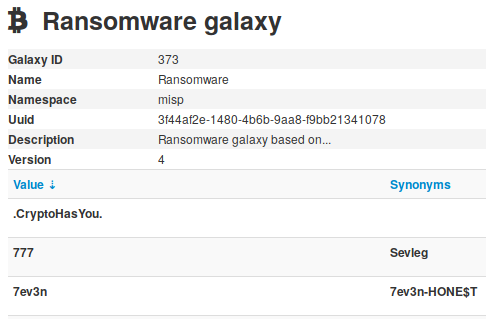
\includegraphics[scale=0.30]{galaxy-ransomware.png}
    \end{center}
\end{frame}

\begin{frame}
  \frametitle{The emergence of ATT\&CK and similar galaxies}
  \begin{itemize}
    \item Standardising on high-level {\bf TTPs} was a solution to a long list of issues
    \item Adoption was rapid, tools producing ATT\&CK data, familiar interface for users
    \item A much better take on kill-chain phases in general
    \item Feeds into our {\bf filtering} and {\bf situational awareness} needs extremely well
    \item Gave rise to other, ATT\&CK-like systems tackling other concerns
    \begin{itemize}
      \item {\bf attck4fraud} \footnote{\url{https://www.misp-project.org/galaxy.html\#_attck4fraud}} by Francesco Bigarella from ING
      \item {\bf Election guidelines} \footnote{\url{https://www.misp-project.org/galaxy.html\#_election_guidelines}} by NIS Cooperation Group
    \end{itemize}
  \end{itemize}
\end{frame}

\section{Data that tells a story}

\begin{frame}
  \frametitle{More complex data-structures for a modern age}
  \begin{itemize}
    \item Atomic attributes were a great starting point, but lacking in many aspects
    \item {\bf MISP objects}\footnote{\url{https://github.com/MISP/misp-objects}} system
    \begin{itemize}
      \item Simple {\bf templating} approach
      \item Use templating to build more complex structures
      \item Decouple it from the core, allow users to {\bf define their own} structures
      \item MISP should understand the data without knowing the templates
      \item Massive caveat: {\bf Building blocks have to be MISP attribute types}
      \item Allow {\bf relationships} to be built between objects
    \end{itemize}
  \end{itemize}
\end{frame}

\begin{frame}
  \frametitle{Supporting specific datamodels}
  \begin{center}
    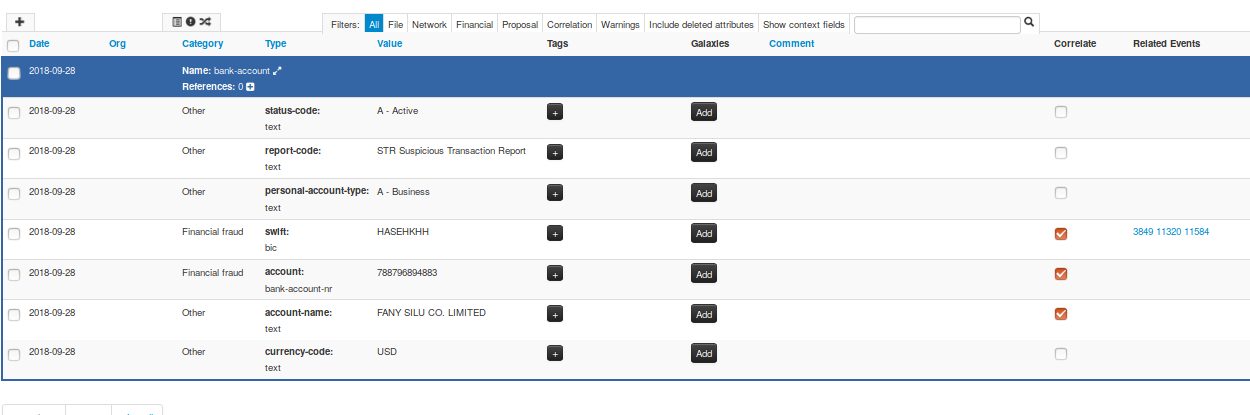
\includegraphics[scale=0.24]{bankaccount.png}
  \end{center}
  \begin{center}
    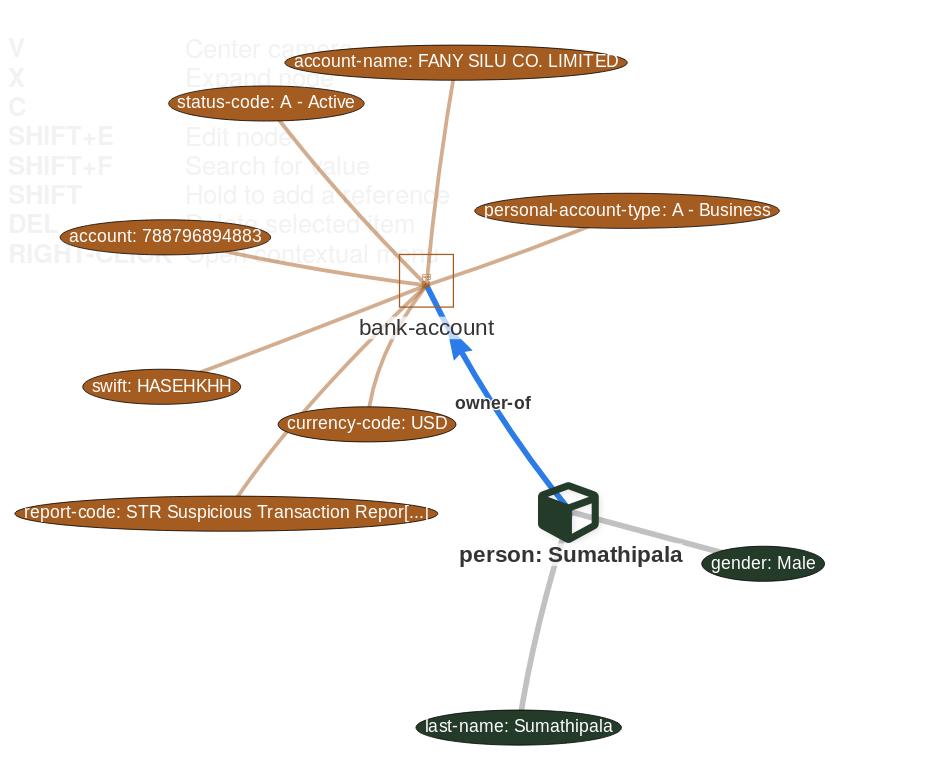
\includegraphics[scale=0.18]{bankview.png}
  \end{center}
\end{frame}

\begin{frame}
  \frametitle{Continuous feedback loop}
  \begin{itemize}		  
    \item Data shared was {\bf frozen in time}
    \item All we  had was a creation/modification timestamp
    \item Improved tooling and willingness allowed us to create a {\bf feedback loop}
    \item Lead to the introduction of the {\bf Sighting system}
    \item Signal the fact of an indicator sighting...
    \item ...as well as {\bf when} and {\bf where} it was sighted
    \item Vital component for IoC {\bf lifecycle management}
  \end{itemize}
\end{frame}

\begin{frame}
  \frametitle{Continuous feedback loop (2)}
  \begin{center}
    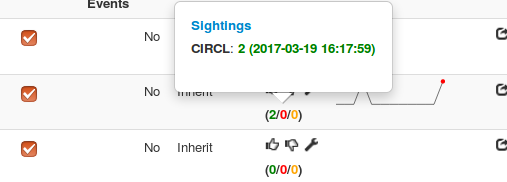
\includegraphics[scale=0.5]{sighting-n.png}
  \end{center}
  \begin{center}
    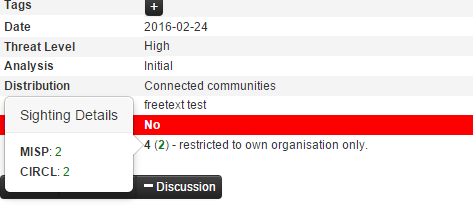
\includegraphics[scale=0.60]{Sightings2.PNG}
  \end{center}  
\end{frame}

\begin{frame}
  \frametitle{A brief history of time - Adding temporality to our data}
  \begin{itemize}
    \item As Andreas said - no time based aspect was painful
    \item Recently introduced {\bf \texttt{first\_seen}} and {\bf \texttt{last\_seen}} data points
    \item Along with a complete integration with the {\bf UI}
    \item Enables the {\bf visualisation} and {\bf adjustment} of indicators timeframes 
  \end{itemize}
  \begin{center}
    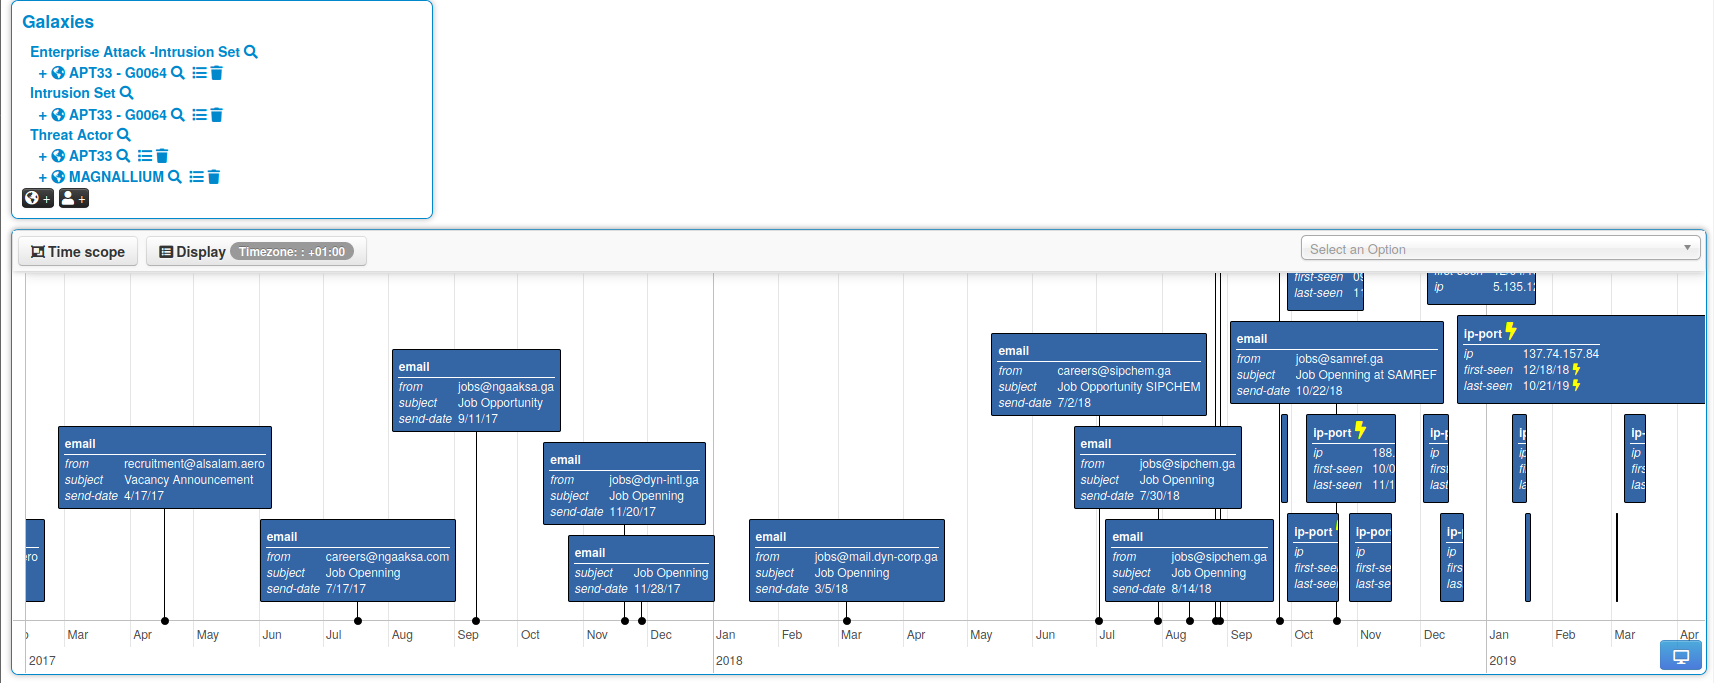
\includegraphics[width=1.0\linewidth]{timeline-misp-overview.png}
  \end{center}
\end{frame}

\section{The various ways of encoding analyst knowledge to automatically leverage our TI}

\begin{frame}
\frametitle{False positive handling}
\begin{itemize}
        \item Low quality / false positive prone information being shared
        \item Lead to {\bf alert-fatigue}
        \item Exclude organisation xy out of the community?
        \item FPs are often obvious - {\bf can be encoded}
        \item {\bf Warninglist system}\footnote{\url{https://github.com/MISP/misp-warninglists}} aims to do that
        \item Lists of well-known indicators which are often false-positives like RFC1918 networks, ...
\end{itemize}
\begin{center}
    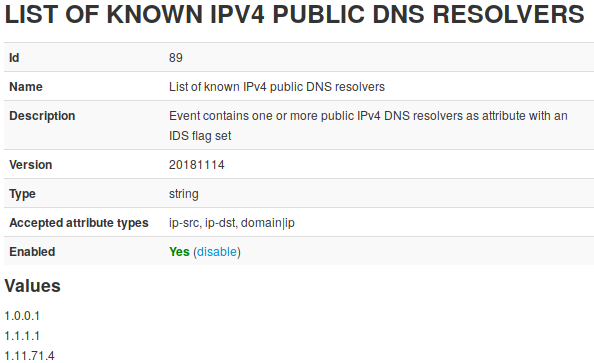
\includegraphics[scale=0.22]{warning-list.png}
    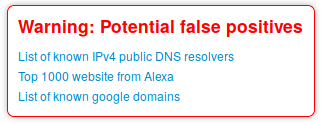
\includegraphics[scale=0.45]{warning-list-event.png}
\end{center}
\end{frame}

\begin{frame}
  \frametitle{Making use of all this context}
  \begin{itemize}
    \item Providing advanced ways of querying data
    \begin{itemize}
      \item Unified export APIs
      \item Incorporating all contextualisation options into {\bf API filters}
      \item Allowing for an {\bf on-demand} way of {\bf excluding potential false positives}
      \item Allowing users to easily {\bf build their own} export modules feed their various tools
    \end{itemize}
  \end{itemize}
\end{frame}

\begin{frame}[fragile]
    \frametitle{Example query}
    \texttt{/attributes/restSearch}
    \begin{lstlisting}
{
    "returnFormat": "netfilter",
    "enforceWarninglist": 1,
    "tags": {
      "NOT": [
        "tlp:white",
        "type:OSINT"
      ],
      "OR": [
        "misp-galaxy:threat-actor=\"Sofacy\"",
        "misp-galaxy:sector=\"Chemical\""
      ],
    }
}
    \end{lstlisting}
\end{frame}

\begin{frame}[fragile]
    \frametitle{Example query to generate ATT\&CK heatmaps}
    \texttt{/events/restSearch}
    \begin{lstlisting}
{
    "returnFormat": "attack",
    "tags": [
        "misp-galaxy:sector=\"Chemical\""
    ],
    "timestamp": "365d"
}
    \end{lstlisting}
\end{frame}

\begin{frame}
  \frametitle{A sample result for the above query}
  \begin{center}
    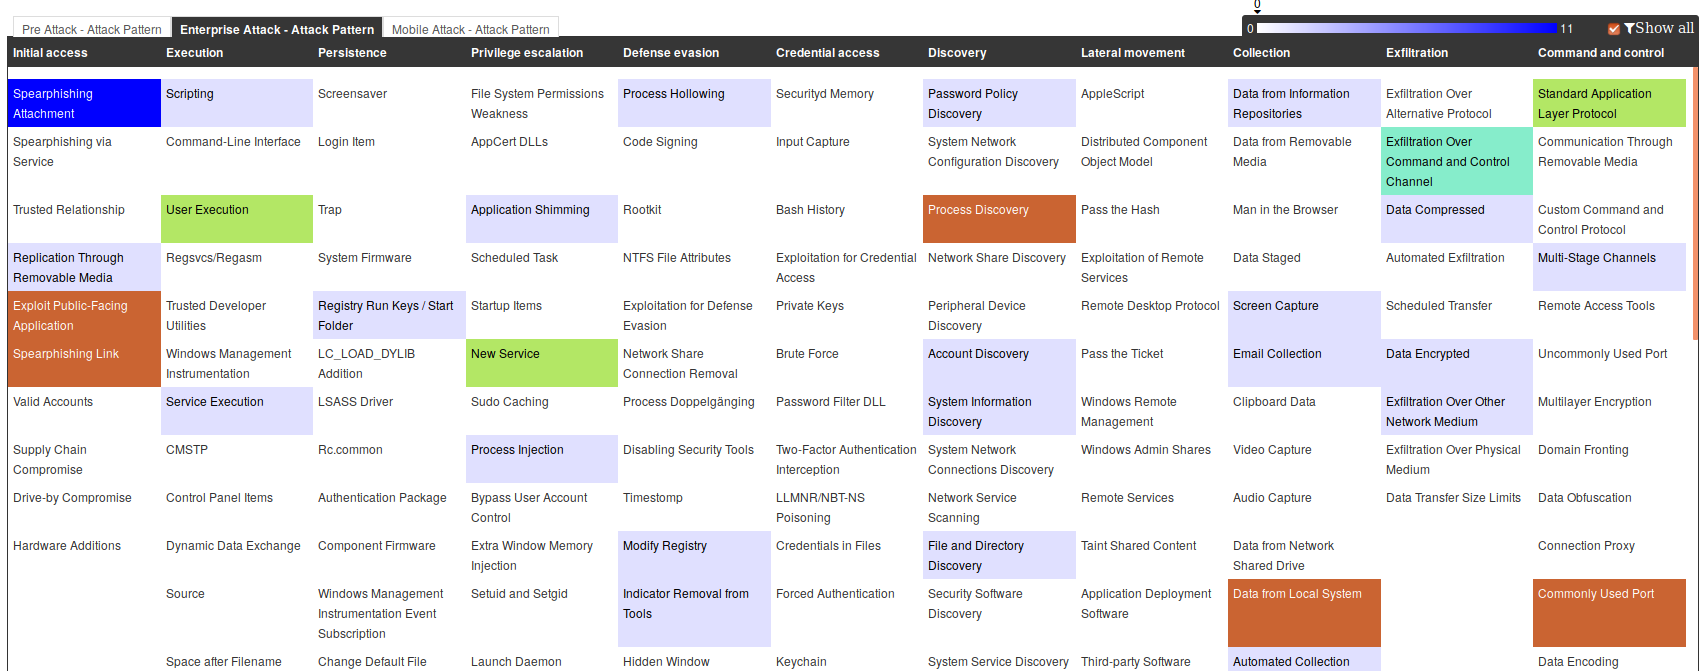
\includegraphics[scale=0.2]{attack-screenshot.png}
  \end{center}
\end{frame}

\begin{frame}
  \frametitle{Monitor trends outside of MISP (example: dashboard)}
  \begin{center}
    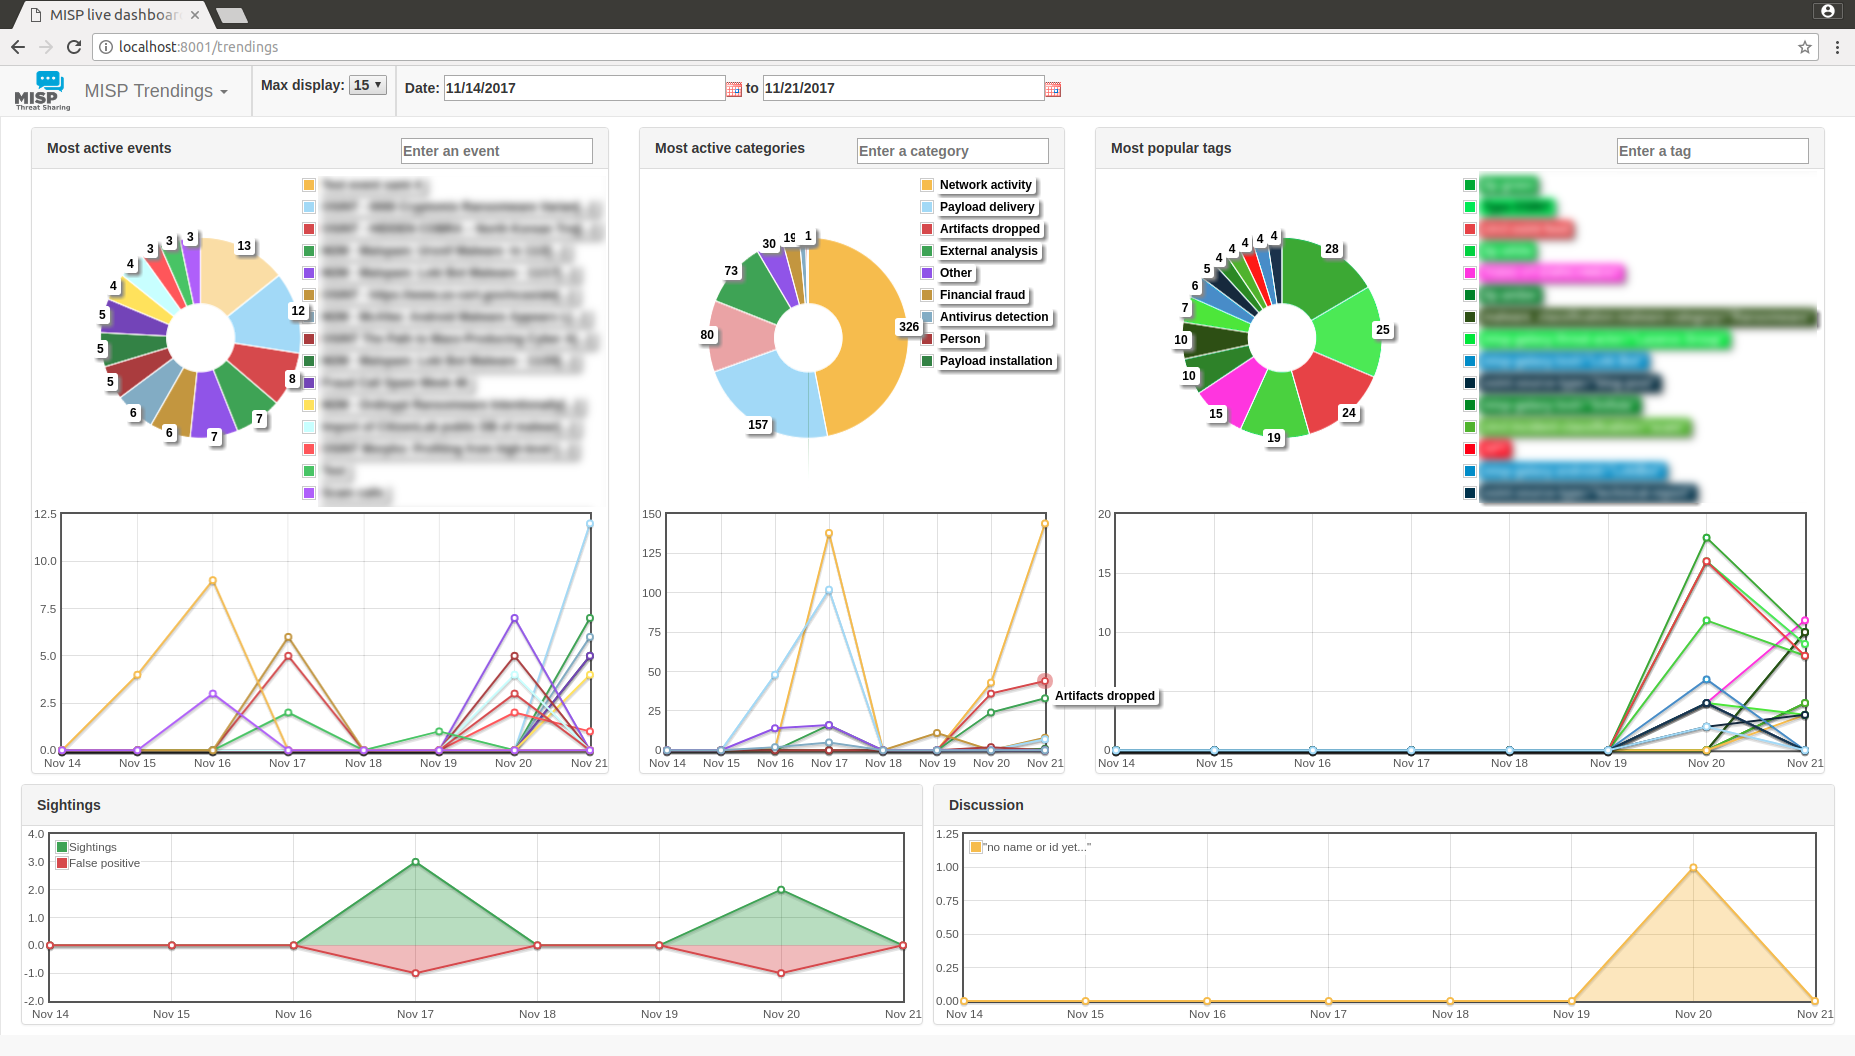
\includegraphics[scale=0.2]{dashboard-trendings.png}
  \end{center}
\end{frame}

\begin{frame}
  \frametitle{Decaying of indicators}
  \begin{itemize}
    \item We were still missing a way to use all of these systems in combination to decay indicators
    \item Move the decision making \textbf{from complex filter options to} complex \textbf{decay models}
    \item Decay models would take into account various available {\bf context}
    \begin{itemize}
      \item Taxonomies
      \item Sightings
      \item type of each indicator
      \item Creation date
      \item ...
    \end{itemize}
  \end{itemize}
\end{frame}

\begin{frame}
    \frametitle{Implementation in MISP: \texttt{Event/view}}
    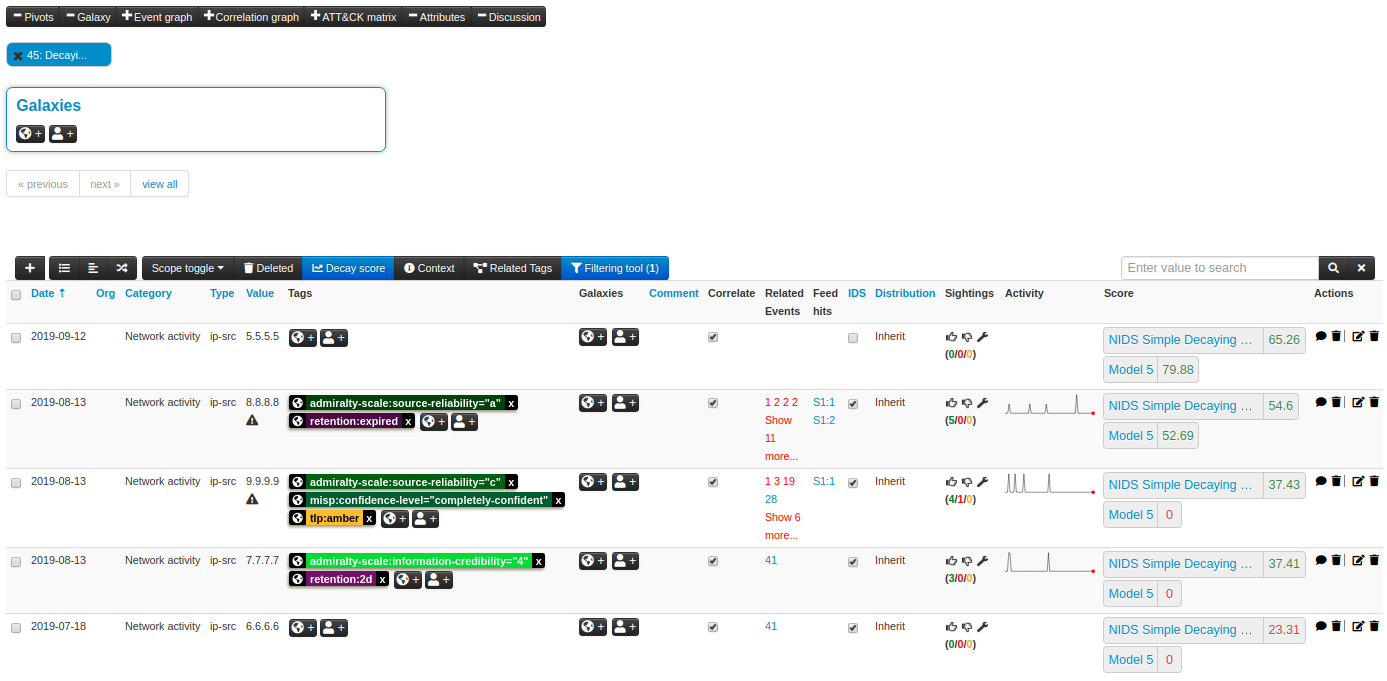
\includegraphics[width=1.00\linewidth]{decaying-event.png}
    \begin{itemize}
        \item \texttt{Decay score} toggle button
        \begin{itemize}
            \item Shows Score for each \textit{Models} associated to the \textit{Attribute} type
        \end{itemize}
    \end{itemize}
\end{frame}

\begin{frame}[fragile]
    \frametitle{Implementation in MISP: API result}
    \texttt{/attributes/restSearch}
    \begin{lstlisting}
"Attribute": [
  {
    "category": "Network activity",
    "type": "ip-src",
    "to_ids": true,
    "timestamp": "1565703507",
    [...]
    "value": "8.8.8.8",
    "decay_score": [
      {
        "score": 54.475223849544456,
        "decayed": false,
        "DecayingModel": {
          "id": "85",
          "name": "NIDS Simple Decaying Model"
        }
      }
    ],
[...]
    \end{lstlisting}
\end{frame}


\begin{frame}
  \frametitle{To sum it all up...}
  \begin{itemize}
     \item Massive rise in {\bf user capabilities}
     \item Growing need for truly {\bf actionable threat intel}
     \item Lessons learned:
     \begin{itemize}
	\item {\bf Context is king} - Enables better decision making
        \item {\bf Intelligence and situational awareness} are natural by-products of context
        \item Don't lock users into your {\bf workflows}, build tools that enable theirs
     \end{itemize}
  \end{itemize}
\end{frame}

\begin{frame}
  \frametitle{Get in touch if you have any questions}
  \begin{itemize}
    \item Contact us
    \begin{itemize}
      \item \url{https://twitter.com/mokaddem_sami}
      \item \url{https://twitter.com/iglocska}
    \end{itemize}
    \item Contact CIRCL
    \begin{itemize}
      \item info@circl.lu
      \item \url{https://twitter.com/circl_lu}
      \item \url{https://www.circl.lu/}
    \end{itemize}
    \item Contact MISPProject 
    \begin{itemize}
      \item \url{https://github.com/MISP}
      \item \url{https://gitter.im/MISP/MISP}
      \item \url{https://twitter.com/MISPProject}
    \end{itemize}
  \end{itemize}
\end{frame}
